\chapter{Estado del arte}
Estos son los entornos que conforman el estado del arte en entornos para el aprendizaje por refuerzo con múltiples agentes. Algunos de los entornos siguientes serán descartados por no tener el código disponible o por otros factores. Además, los candidatos restantes serán valorados con las métricas especificadas en el apartado anterior para decidir cuál adaptaremos en este trabajo. Otro aspecto a tener en cuenta es que dividiremos los entornos en los que ya sirven para entrenar agentes de por sí (entornos funcionales) y los que deben adaptarse (entornos para adaptación).  

\section{Entornos funcionales}

Hay que tener en cuenta que por norma general, la mayoría de estos entornos dispone de buena documentación, ya que se han usado en investigaciones.

\begin{itemize}
	\item \textbf{Neural MMO} \cite{neural-mmo-repo} está basado en el género de gaming MMORPGs (massively multiplayer online role-playing games). El entorno consiste en un mapa autogenerado de tamaño configurable formado por de celdas. Las celdas existentes son de bosque, de hierba, de agua y de roca pura. Solo las celdas de bosque y de hierba son transitables mientras que las de agua y roca no lo son. Estas últimas sirven como obstáculos en el terreno.  

	      El objetivo del entorno es mantenerse vivos durante el mayor número de rondas. Para ello deben recolectar comida y agua y evitar recibir daño de otros agentes. Para obtener comida deben colocarse encima de una celda de bosque. Estas celdas tienen una cantidad de comida limitada que se rellena lentamente, por lo que los agentes deberán competir por este recurso. A diferencia de la comida, obtener agua es simple, simplemente deben estar al lado de una celda de agua y las reservas de agua son infinitas. Podemos ver la representación del entorno en la figura \ref {fig:neural-mmo-2}.  

	      Los agentes se dividen en 3 categorías distintas, cuerpo a cuerpo, a distancia y mago. Estas categorías marcan la forma de atacar de cada agente.
	      El \textbf{input} consiste en las celdas colindantes a la posición de cada agente así como a la vida, comida y agua de los agentes que ocupen estas celdas. El \textbf{output} consiste en un movimiento y un ataque. 

	      Las características que hemos podido identificar este entorno son las siguientes:
	      \begin{itemize}
		      \item El entorno obliga a la competición aunque también puede existir la cooperación más no es obligatoria.
		      \item Es un entorno muy bien documentado por ser de una compañía grande (OpenAI) \cite {openia}
		      \item Los agentes aprenden en el entorno sin resets, así que se deben considerar estrategias a largo plazo haciendo que el entorno sea más rico.
		      \item No está limitado a un cierto número de agentes.
		      \item Este entorno sigue la filosofía de construcción de entornos de Gym de OpenAI.
		      \item El proyecto ha sido abandonado por la compañía así que no recibe más actualizaciones ni mantenimiento.
		      \item El objetivo del entorno es monótono.
		      \item Puesto que el entorno está enfocado a ser de gran escala tiene un gran coste computacional.
	      \end{itemize}

	      \begin{figure}[ht]
		      \centering
		      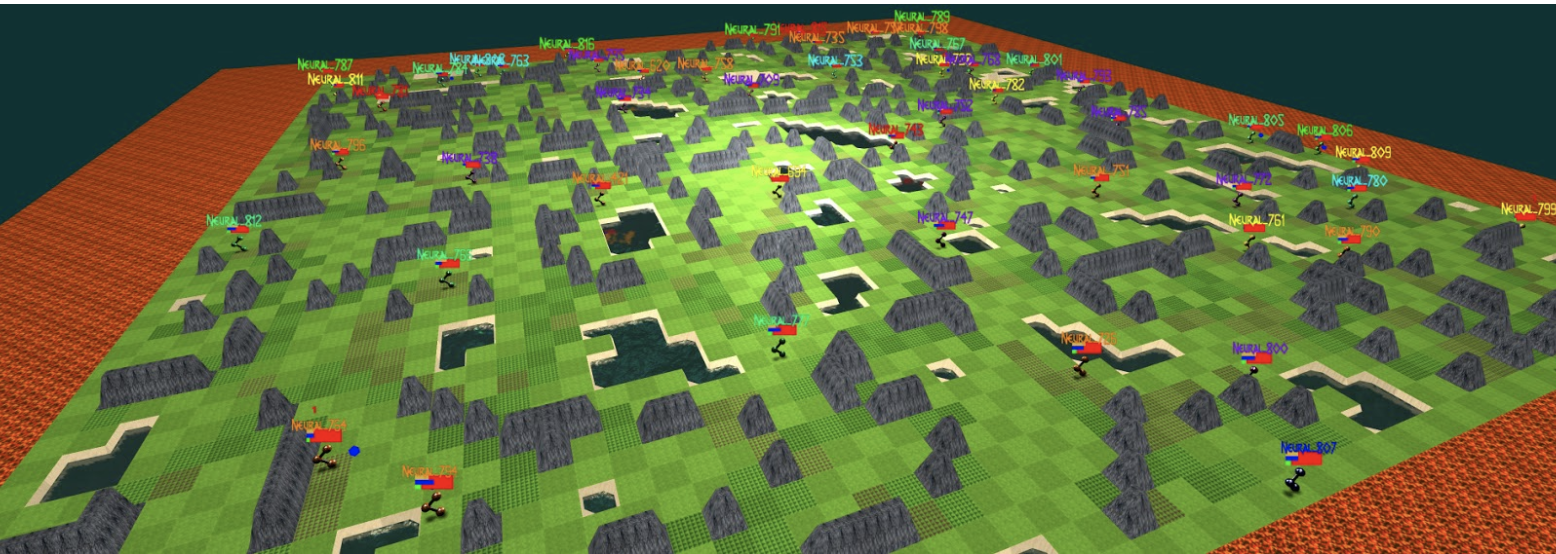
\includegraphics[width=0.7\textwidth]{img/neural-mmo.png}
		      \caption{Entorno gráfico 3D de Neural MMO \cite{neural-mmo}}
		      \label{fig:neural-mmo-2}
	      \end{figure}

	\item \textbf{Level-Based Foraging} \cite {level-based-repo} es un entorno que consiste en un conjunto de tareas que pueden ser cooperativas o competitivas que se centran especialmente en la coordinación entre agentes. En todas las tareas los agentes deben navegar por una cuadrícula de celdas y recolectar objetos. Los ítems se reparten aleatoriamente por la cuadrícula. A los agentes y los ítems se les asigna un nivel.  Para poder recolectar un ítem, el nivel de los agentes que lo recogen debe ser igual o mayor al nivel del ítem. El nivel del ítem se corresponde con la recompensa de los agentes. Por lo tanto el objetivo del entorno es conseguir la mayor recompensa posible. Este entorno incorpora cierta coordinación entre agentes, puesto que muchos objetos solo se podrán obtener cuando dos o más agentes lo intenten coger a la vez. En la figura \ref {fig:foraging} podemos ver la visualización de las diferentes tareas del entorno.  

	      Por defecto los agentes pueden ver el mapa entero y las posiciones del resto de agentes, pero también existen tareas donde la visibilidad es parcial. El \textbf{input}, si se trata de una tarea de visibilidad total, consiste en la cuadrícula con la posición de todos los agentes y los objetos junto con la información del nivel. Si se trata de una tarea de visibilidad parcial entonces el input consiste en una cuadrícula más pequeña que el mapa entero centrado en el agente en cuestión. El \textbf{output} consiste en un movimiento en cualquiera de las cuatro direcciones o el intento de coger un ítem.  

	      Las características que hemos podido identificar este entorno son las siguientes:
	      \begin{itemize}
		      \item El entorno obliga a la cooperación.
		      \item El entorno no está limitado a un cierto número de agentes.
		      \item Sigue el paradigma de entornos de Gym.
	      \end{itemize}

	      \begin{figure}[h]
		      \centering
		      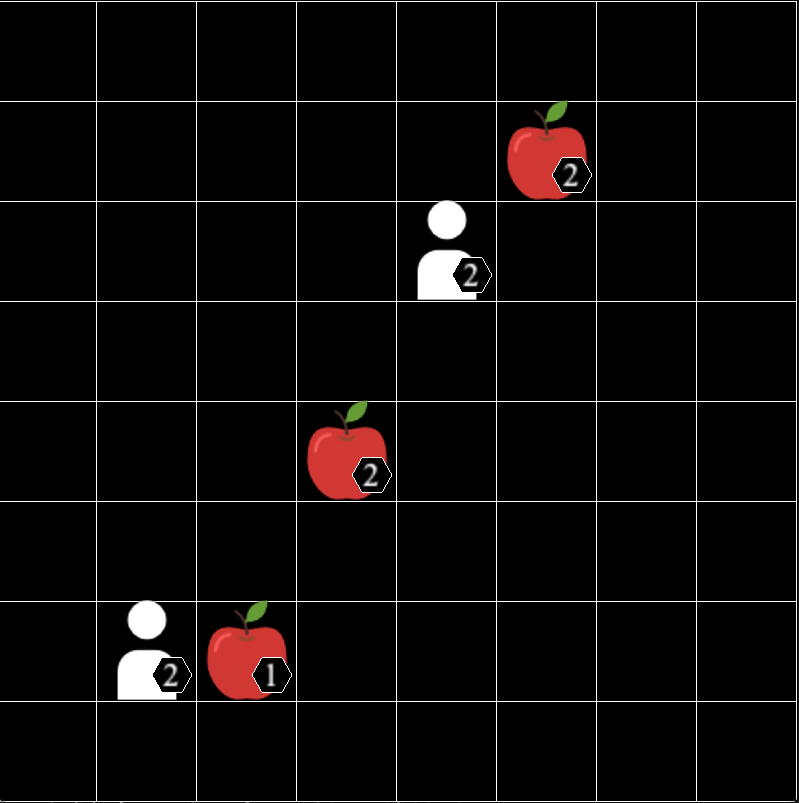
\includegraphics[width=0.3\textwidth]{img/level-base.png}
		      \caption{Entorno gráfico de Level-Based Foraging \cite {env-list}}
		      \label{fig:foraging}
	      \end{figure}

	\item \textbf{PressurePlate} \cite {pressure-repo} es un entorno multiagente basado en el entorno Level-Base Foraging que requiere que los agentes cooperen durante la travesía del mapa. El mapa por el que se mueven los agentes es una cuadrícula separada por diferentes habitaciones conectadas entre ellas por una puerta. Para poder abrir la puerta y cruzar a la siguiente habitación es necesario que alguno de los agentes se coloque encima de la placa de presión de la habitación. Al principio de la tarea, a cada agente se le asigna una placa que deben presionar. Por lo tanto los agentes deben moverse a través de la secuencia de habitaciones dejando en cada habitación al agente asignado a la placa de esa habitación permitiendo pasar al resto del grupo. La tarea se considera solucionada una vez un agente ha llegado al último objetivo marcado como un cofre. En la figura \ref {fig:pressure} podemos ver la visualización de un ejemplo de tarea del entorno.  

	      Las recompensas de este entorno son densas, ya que se otorgan en función de la distancia de un agente y la placa de presión asignada. De esta forma, las recompensas son individuales, pero los agentes deben de cooperar para conseguirlas. El \textbf{input} de esta tarea es similar al de Level-Base Foraging añadiendo además la existencia de paredes, puertas y placas de presión. El \textbf{output} es completamente igual al del entorno en el que está basado. 

	      Las características que hemos podido identificar este entorno son las siguientes:
	      \begin{itemize}
		      \item El entorno obliga a la cooperación entre agentes.
		      \item El entorno no está limitado a un cierto número de agentes.
		      \item Es posible crear mapas personalizados.
		      \item Sigue el paradigma de entornos de Gym.
	      \end{itemize}

	      \begin{figure}[h]
		      \centering
		      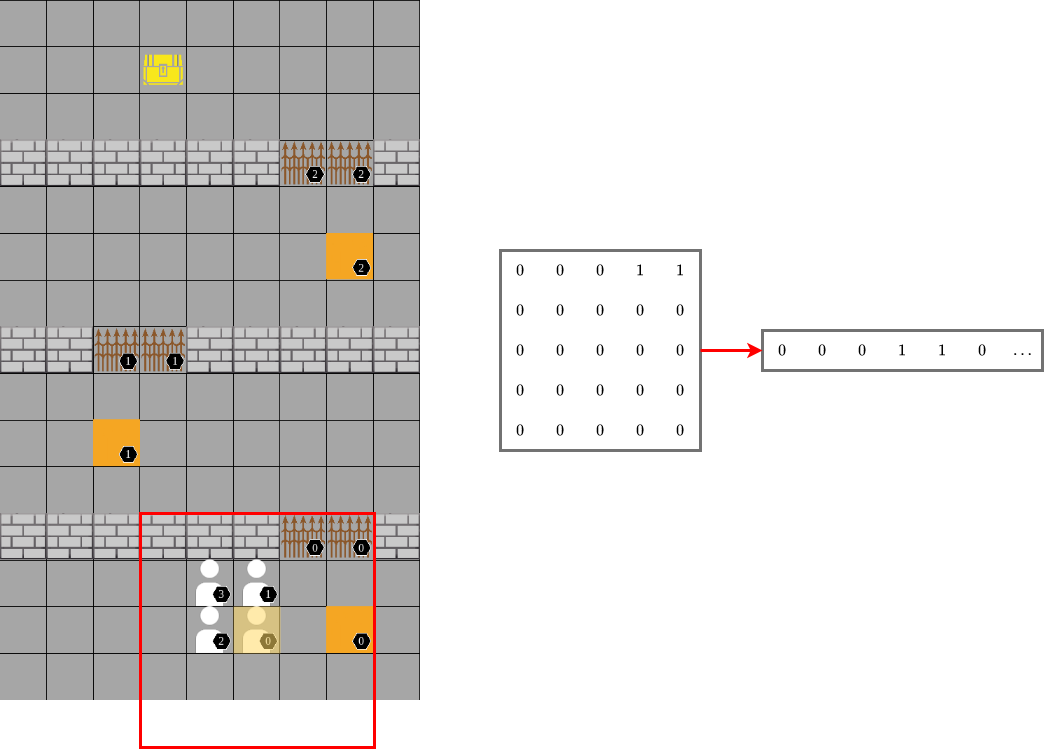
\includegraphics[width=0.5\textwidth]{img/obs_example.png}
		      \caption{Entorno gráfico de PressurePlate con la codificación de la información para los agentes \cite {env-list}}
		      \label{fig:pressure}
	      \end{figure}

	\item \textbf{Multi-Robot Warehouse} \cite {warehouse-repo} es un entorno que simula un depósito con robots moviendo mercancías. Este entorno está basado en situaciones de la vida real donde los robots cargan una bandeja desde una estantería a un punto en concreto donde un operario evalúa el contenido de la esta. Una vez realizado la evaluación, el robot devuelve la bandeja a una estantería libre. Por lo tanto, el objetivo del entorno es revisar el número máximo de bandejas teniendo en cuenta que es necesario devolver la bandeja que se ha revisado a un hueco libre en la estantería. El movimiento en este entorno es interesante, puesto que los robots pueden pasar por debajo de las estanterías mientras no carguen una bandeja. En la figura \ref {fig:warehouse} podemos ver la representación gráfica del entorno.  

	      El \textbf{input} consiste en una cuadrícula de 3 x 3 celdas centradas en la  ubicación de cada agente junto con la información de los agentes y estanterías situados en estas celdas. El \textbf{output} consiste en rotar el robot a izquierda o derecha, avanzar y cargar o descargar una bandeja. En cada momento se solicitan un cierto número de bandejas, este valor está relacionado con el número de robots y cambia en función de la dificultad que se haya seleccionado. El entorno de base tiene tres mapas de distinto tamaño y tres variaciones de dificultad que varían el número de bandejas solicitadas. Como medida de rendimiento se usa la suma de todas las bandejas entregadas por todos los agentes, puesto que se trata de una tarea colaborativa.  

	      Las características que hemos podido identificar este entorno son las siguientes:
	      \begin{itemize}
		      \item Sigue el paradigma de entornos de Gym.
		      \item El entorno no está limitado a un cierto número de agentes.
	      \end{itemize}

	      \begin{figure}[ht]
		      \centering
		      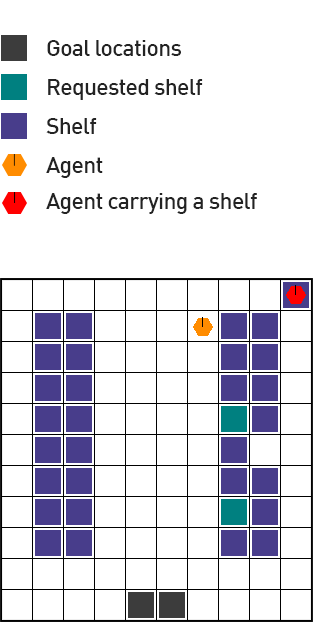
\includegraphics[width=0.3\textwidth]{img/rware-tiny.png}
		      \caption{Entorno gráfico de Multi-Robot Warehouse \cite {env-list}}
		      \label{fig:warehouse}
	      \end{figure}

	\item \textbf{Multi-Agent Particle Environment} \cite {particle-repo} Es un entorno con una gran variedad de tareas de coordinación y competición. En todas las tareas los agentes que son representados por partículas interactúan entre ellos y con puntos de referencia en el mapa para conseguir sus objetivos. Los objetivos de las tareas varían mucho así que daremos algunos ejemplos:

	      \begin{itemize}
		      \item \textbf{Speaker-Listener}: Se trata de una tarea cooperativa donde una partícula completamente estática tiene que comunicar a otra partícula móvil la posición de un punto de referencia objetivo. En total hay 3 puntos de referencia en el entorno y ambos agentes son recompensados entre menor sea la distancia de la partícula móvil al punto de referencia objetivo. La partícula estática solo puede observar el color del punto de referencia objetivo mientras que la partícula móvil recibe su propia velocidad, la distancia a todos los puntos de referencia y la comunicación de la partícula estática. La partícula móvil puede realizar movimientos en cualquiera de las 4 direcciones o dejarse de mover mientras que la partícula estática posee tres tipos de acciones de comunicación. En la figura \ref {fig:speaker-listener} podemos observar como se ve la tarea gráficamente.

		            \begin{figure}[ht]
			            \centering
			            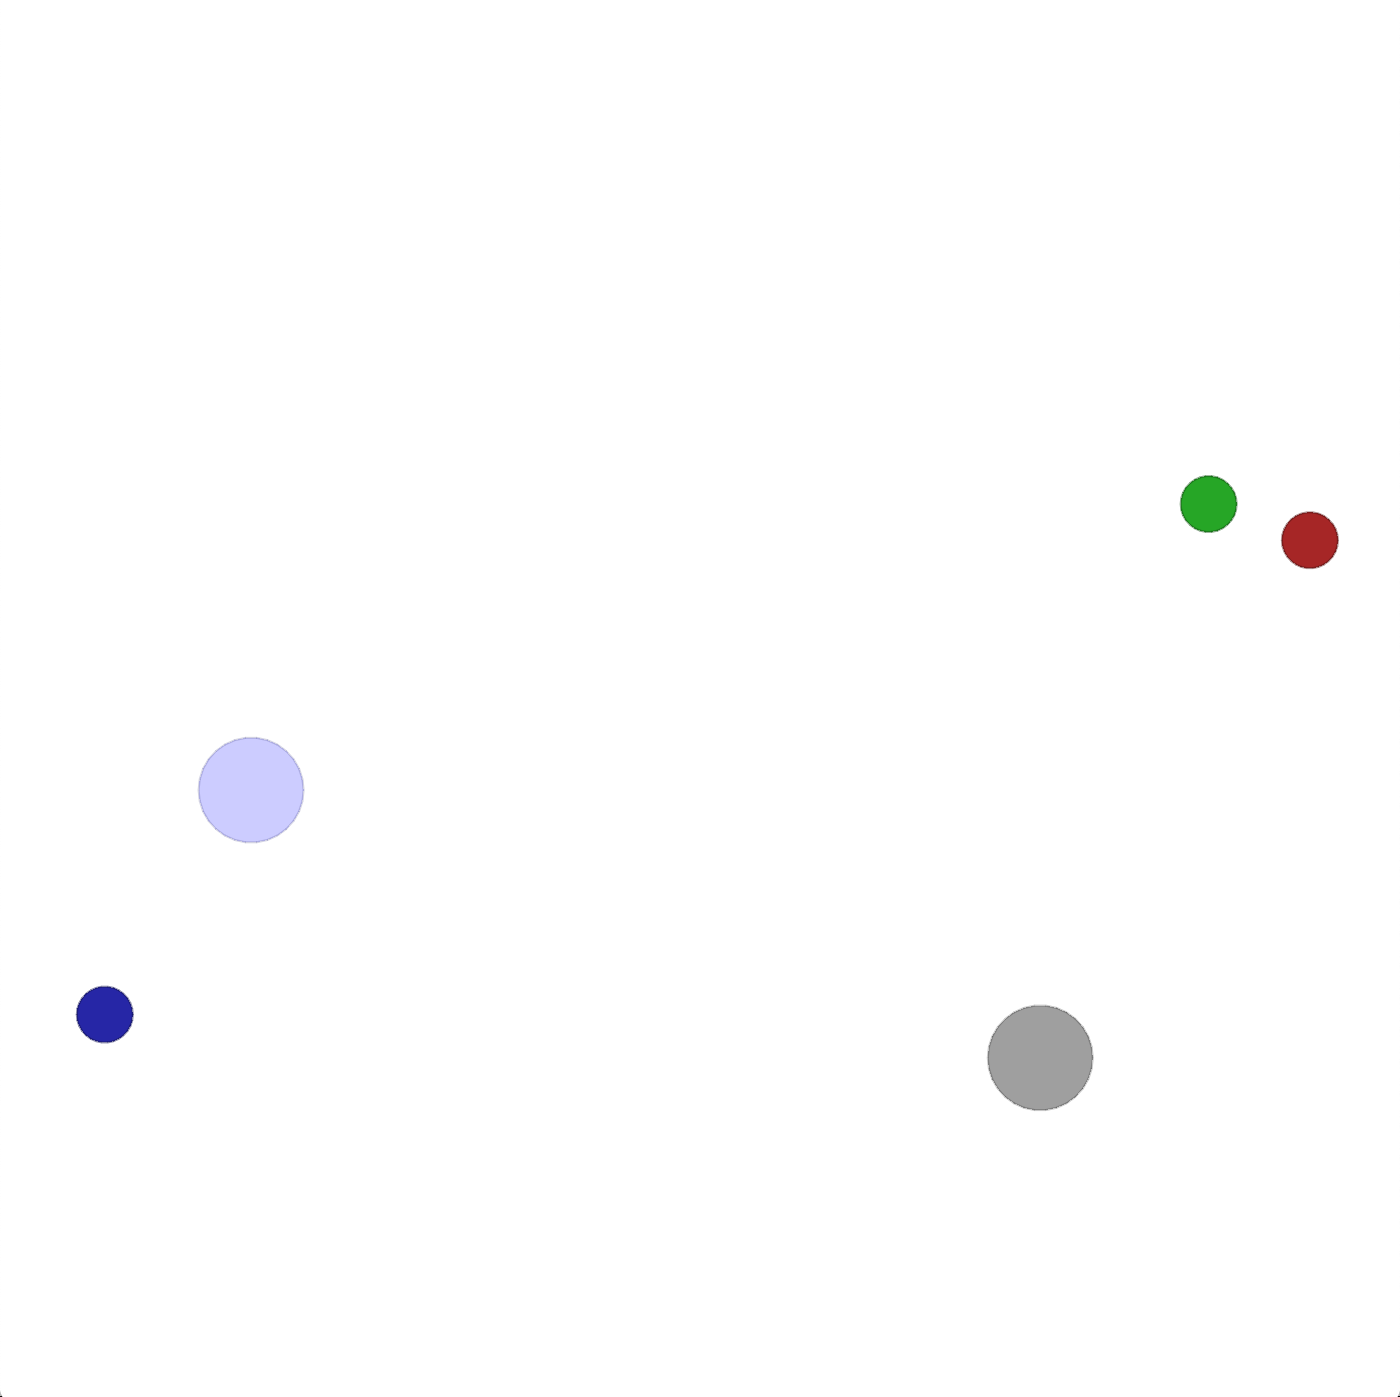
\includegraphics[width=0.3\textwidth]{img/mape_simple_speaker_listener.png}
			            \caption{Entorno gráfico de Multi-Agent Particle Environment en la tarea de Speaker-Listener. Los puntos más grandes corresponden a partículas mientras que los más pequeños a puntos de referencia \cite{ env-list}}
			            \label{fig:speaker-listener}
		            \end{figure}
		      \item \textbf{Predator-Prey}: Se trata de una tarea competitiva donde 3 agentes que hacen el rol de depredador cazan a un cuatro agente que tiene el rol de presa. En el entorno hay situados dos obstáculos. Todos los agentes reciben su propia velocidad y posición además de la posición del resto de agentes y obstáculos del mapa. Los agentes depredadores también observan la velocidad de la presa. Las acciones de los agentes es el movimiento en cualquiera de las 4 direcciones. El agente que hace de presa recibe penalización por cada colisión con los depredadores y estos reciben bonificación por ello. Para que se pueda observar cierta cooperación entre los agentes depredadores, el agente presa tiene una velocidad mayor a estos, forzándolos a crear estrategias. En la figura \ref {fig:predator-prey} podemos observar como se ve la tarea gráficamente.

		            \begin{figure}[ht]
			            \centering
			            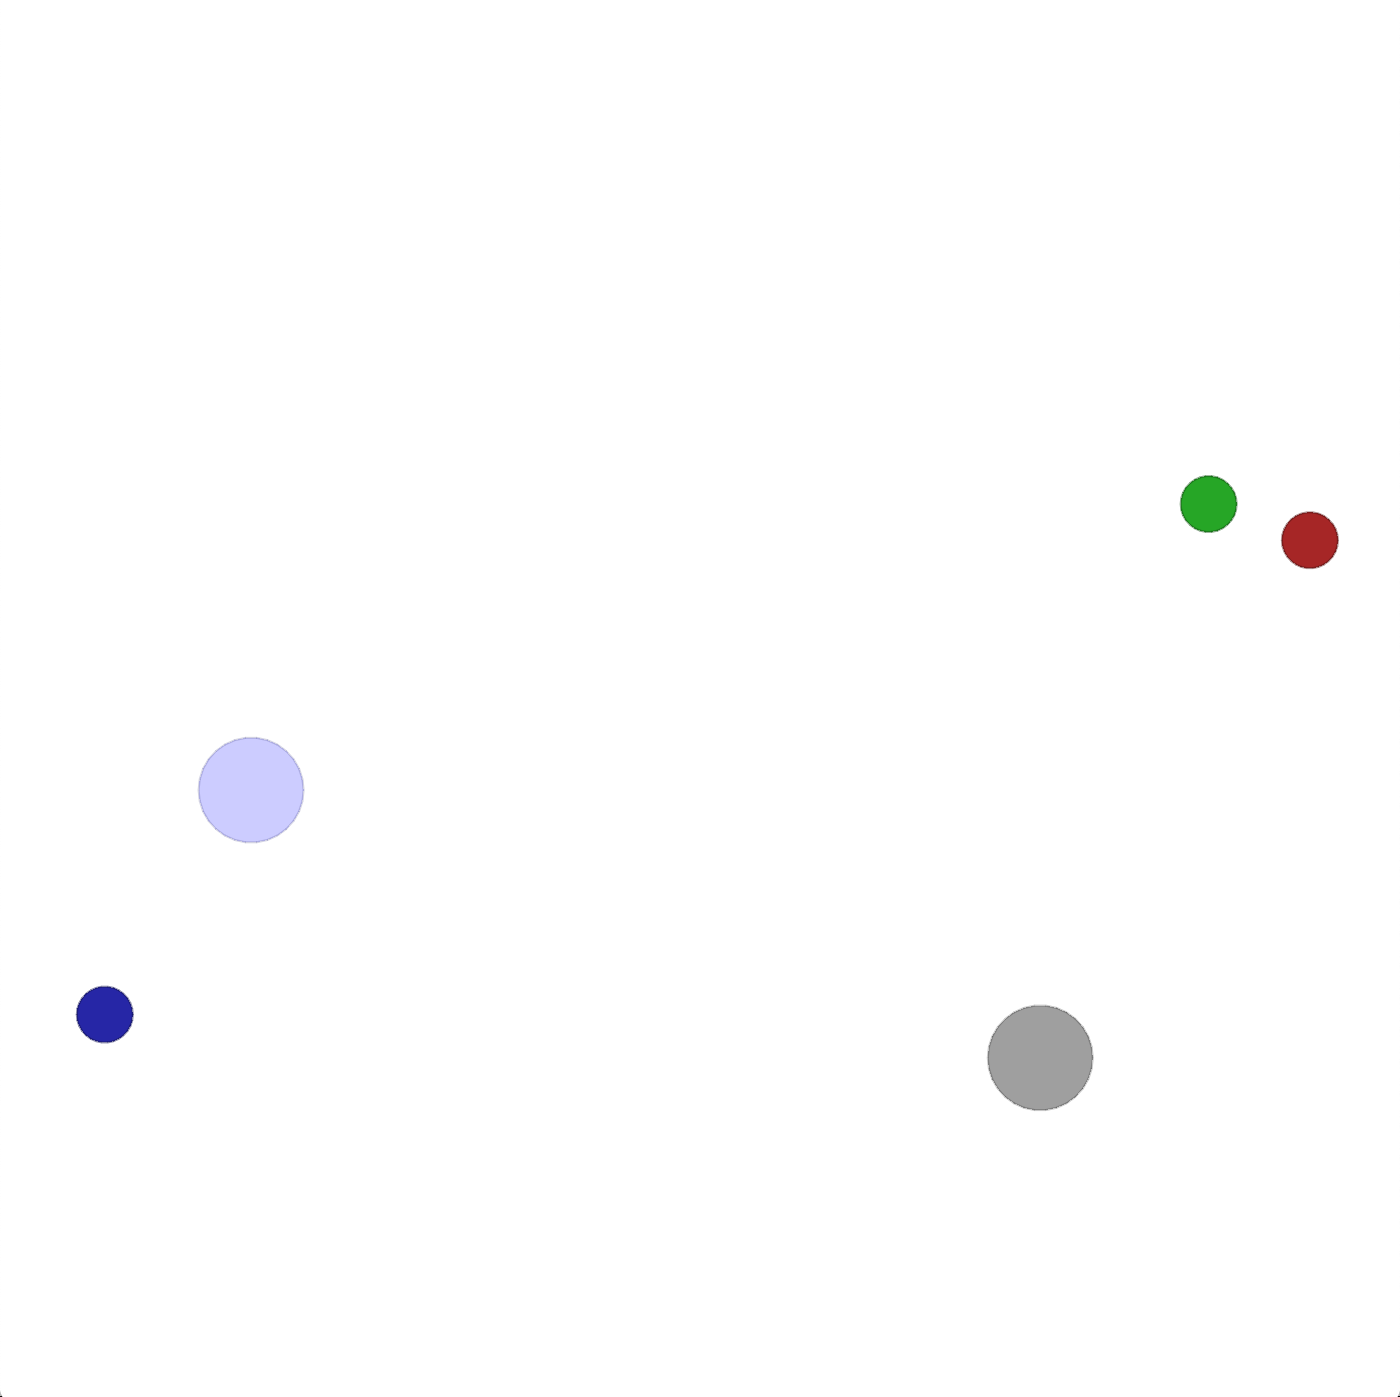
\includegraphics[width=0.3\textwidth]{img/mape_simple_speaker_listener.png}
			            \caption{Entorno gráfico de Multi-Agent Particle Environment en la tarea de Predator-Prey. Los puntos más grandes rojos corresponden a los depredadores mientras que el punto verde corresponde a la presa. Los puntos negros corresponden a obstáculos \cite {env-list}}
			            \label{fig:predator-prey}
		            \end{figure}
	      \end{itemize}
	      Viendo los ejemplos anteriores podemos extrapolar que normalmente el \textbf{input} consiste en la posición del resto de partículas y en el entorno además de la velocidad del agente. El \textbf{output} suele consistir en un movimiento en cualquiera de las cuatro direcciones aunque a veces también puede incluir acciones de comunicación. 

	      Las características que hemos podido identificar este entorno son las siguientes:
	      \begin{itemize}
		      \item La documentación de las diferentes tareas es extensa y por lo tanto su documentación.
		      \item Sigue el paradigma de entornos de Gym.
		      \item Adaptar este entorno y añadir nuevas tareas es relativamente sencillo.
		      \item Algunas tareas del entorno obligan a competir.
		      \item Algunas tareas del entorno obligan a cooperar.
		      \item Existe en algunas tareas del entorno permiten una comunicación estructurada.
	      \end{itemize}

	\item \textbf{MALMÖ} \cite {malmo} es un entorno basado en el juego de Minecraft. Su mundo 3D contiene un conjunto muy diverso de tareas y sub entornos. Los agentes interactúan con otros agentes y entidades de diversas formas. La idea es que cada agente sea un jugador del videojuego y deba realizar unas tareas determinadas. Además tiene la ventaja de que fue usado en The Malmö Collaborative AI Challenge y esto aportó una gran cantidad de código y nuevos entornos. Asimismo es posible crear nuevas tareas fácilmente usando un formato XML. Este entorno tiene tantas posibilidades que es complicado determinar cuál es el objetivo de las tareas o incluso el output de los agentes, para hacerlo deberíamos observar cada tarea individualmente. El \textbf{input} consiste en los píxeles generados desde su perspectiva del juego. Podemos ver un ejemplo de entorno creado en MALMÖ en la figura \ref {fig:malmo}.
	      \begin{figure}[h]
		      \centering
		      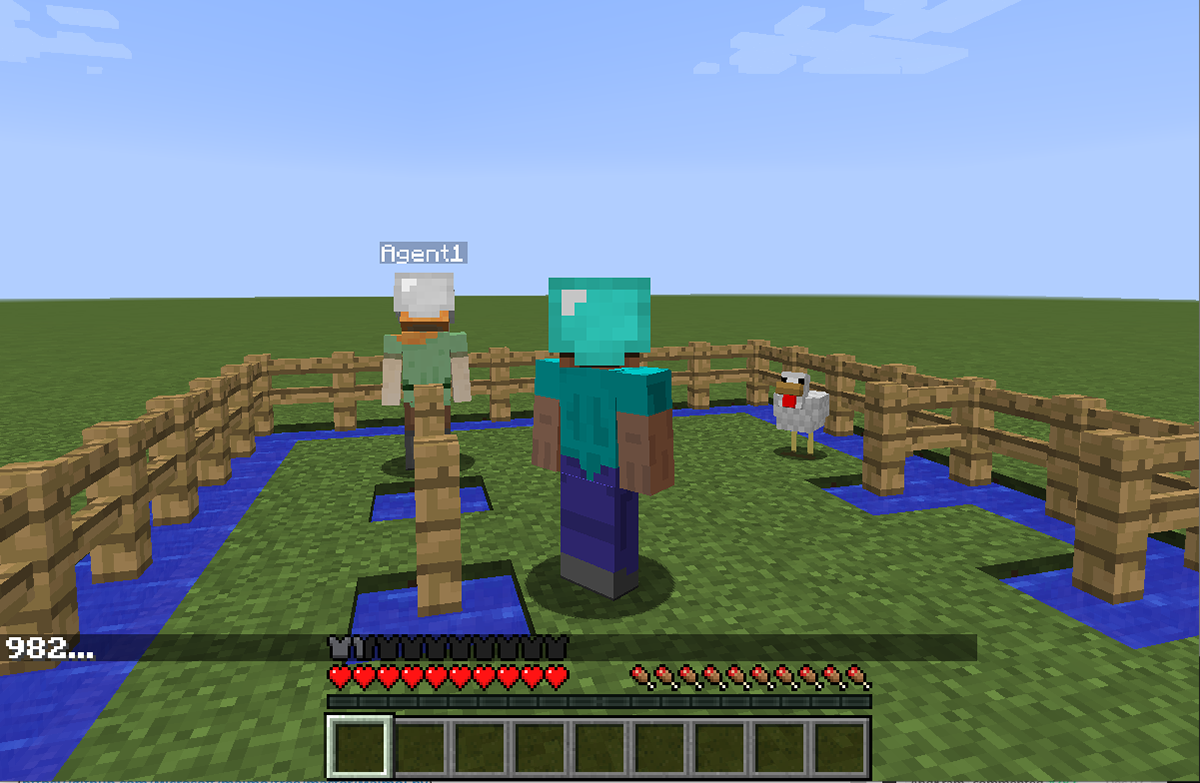
\includegraphics[width=0.5\textwidth]{img/mobchase.png}
		      \caption{Entorno gráfico 3D de MALMÖ en Minecraft. Se puede observar la tarea de capturar al animal \cite {malmo}}
		      \label{fig:malmo}
	      \end{figure}

	      Las características que hemos podido identificar este entorno son las siguientes:
	      \begin{itemize}
		      \item El entorno de Minecraft permite la comunicación por lenguaje natural y algunas de las tareas obligan a la cooperación mientras que otras obligan a la competición.
		      \item Posee una herramienta para definir tareas en XML haciéndolo un procedimiento sencillo.
		      \item Minecraft también permite la negociación.
		      \item El entorno sufre de problemas técnicos y problemas de compatibilidad entre sus distintas tareas.
		      \item Para cada agente debe usarse una instancia distinta de Minecraft que debe conectarse a una red. Este proceso consume muchos recursos además de causar problemas por errores en la conectividad de la red.
		      \item No sigue el paradigma de entornos de Gym.
	      \end{itemize}

	\item \textbf{Pommerman} \cite {pommerman-repo} es un entorno basado en el juego Bomberman. Contiene un mapa en forma de cuadrícula de 11 x 11 donde las tareas que se desarrollan suelen ser la competición de equipos. Los agentes pueden interactuar con el entorno rompiendo las paredes y atacando a otros agentes. Además existe un framework que permite que los agentes de cada equipo se comuniquen entre ellos. Como en el juego Bomberman, al romper una pared existe la posibilidad de obtener un power-up. Los power-ups disponibles son una bomba extra, rango incrementado y la posibilidad de chutar bombas.  

	      El \textbf{input} consiste en la cuadrícula de 11 x 11 aunque también puede utilizarse una observabilidad parcial. Además los agentes tienen la información de su posición, munición, agentes aliados, agentes enemigos entre otros datos. El \textbf{output} consiste en un movimiento en cualquiera de las 4 direcciones además de la acción de colocar una bomba, enviar un mensaje o no hacer nada. En la figura \ref {fig:pommerman} podemos ver la representación del entorno.

	      Las características que hemos podido identificar este entorno son las siguientes:
	      \begin{itemize}
		      \item El entorno obliga a la competición aunque también es posible encontrar cooperación cuando se realizan tareas de equipo.
		      \item El número de agentes está limitado a 4.
		      \item No sigue el paradigma de entornos de Gym.
		      \item Algunas tareas permiten la comunicación estructurada.
	      \end{itemize}

	      \begin{figure}[ht]
		      \centering
		      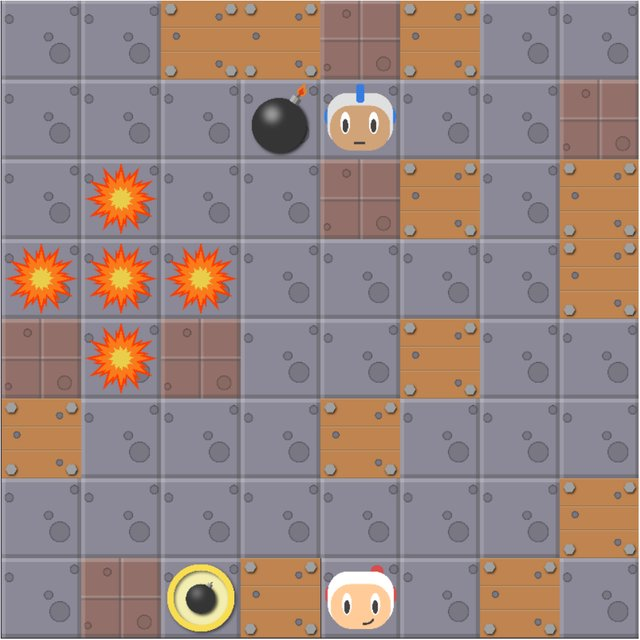
\includegraphics[width=0.3\textwidth]{img/pommerman.jpg}
		      \caption{Entorno gráfico de Pommerman \cite {env-list}}
		      \label{fig:pommerman}
	      \end{figure}

	\item \textbf{Flatland} \cite{flatland-repo} Es un entorno basado en el problema real de coordinar la infraestructura de tráfico de ferroviario de Swiss Federal Railways (SBB). El entorno está representado usando un mapa de cuadrícula y este trata de simular el problema de planificación de los vehículos. Los agentes representan trenes en el sistema de raíles.  

	      El \textbf{input} se puede clasificar en tres tipos posibles en función de como es la de observación del entorno. Puede ser información global de todo el mapa, información local de los alrededores del agente e información en forma de grafo del sistema ferroviario en el estado actual. En la figura \ref {fig:flatland} podemos ver la representación del entorno. El \textbf{output} consiste en las acciones de avanzar, frenar, moverse a izquierda o derecha o no hacer nada. Las recompensas vienen de dos partes distintas, una recompensa global compartida por todos los agentes y una recompensa local por cada agente. El objetivo del entorno es que los trenes lleguen lo más rápido posible a su destino.

	      Las características que hemos podido identificar este entorno son las siguientes:
	      \begin{itemize}
		      \item La documentación del entorno es muy buena.
		      \item Obliga a la cooperación.
		      \item No sigue el paradigma de entornos de Gym.
	      \end{itemize}

	      \begin{figure}[ht]
		      \centering
		      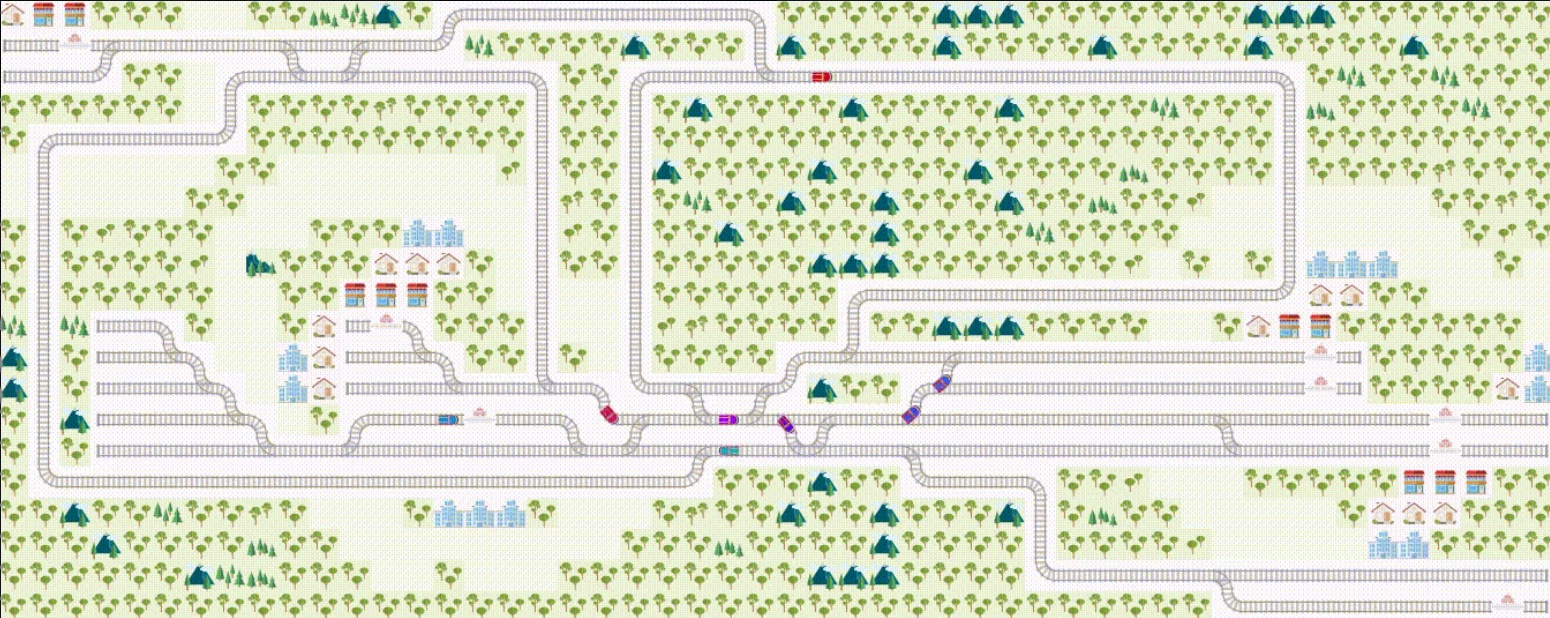
\includegraphics[width=0.7\textwidth]{img/flatland_wide.jpg}
		      \caption{Entorno gráfico de Flatland \cite {env-list}}
		      \label{fig:flatland}
	      \end{figure}

	\item \textbf{Hanabi} \cite{hanabi-repo} Se basa en el juego de cartas Hanabi. Es un entorno completamente cooperativo que puede contener de 2 a 5 agentes donde el principal interés es la cooperación bajo información limitada. Esta información limitada se consigue teniendo una observabilidad parcial. Los jugadores tienen que coordinar sus cartas, pero solo son capaces de ver las cartas de los demás jugadores. Para coordinarse los agentes deben comunicarse entre ellos, pero la comunicación es un recurso limitado en el juego. Además, a diferencia de otros entornos donde todos los agentes actúan a la vez, en este entorno están obligados a actuar por turnos. En la figura \ref {fig:hanabi} podemos ver la representación gráfica del entorno.

	      El \textbf{input} consiste en la información de las cartas del resto de jugadores. El \textbf{output} consiste en dar una pista a otro jugador, jugar una carta de su mano o descartar una carta.

	      Las características que hemos podido identificar este entorno son las siguientes:
	      \begin{itemize}
		      \item Sigue el paradigma de entornos de Gym.
		      \item Obliga a la cooperación entre agentes.
		      \item Permite la comunicación estructurada.
		      \item Está limitado a un cierto número de agentes.
	      \end{itemize}


	      \begin{figure}[ht]
		      \centering
		      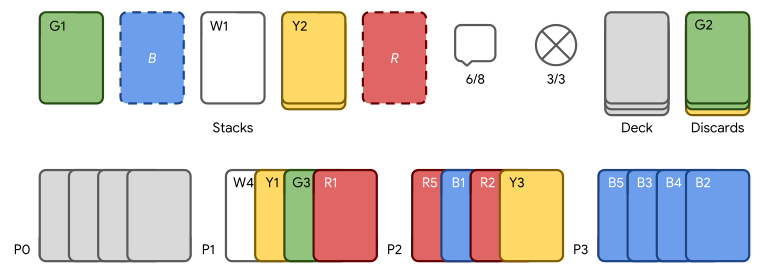
\includegraphics[width=0.7\textwidth]{img/hanabi.png}
		      \caption{Entorno gráfico de Hanabi \cite{env-list}}
		      \label{fig:hanabi}
	      \end{figure}

	\item \textbf{MultiCarRacing} \cite{multicar-repo} Este entorno es un aumento del entorno de Gym CarRacin-v0 \cite {car-repo}. La misión del entorno se basa en una carrera de coches donde los agentes deben aprender a partir de los píxeles de la pantalla. Las acciones sé posibles son acelerar, girar a ambos lados o frenar. Las recompensas se obtienen a partir de un cálculo que tiene en cuenta el número de agentes que han cruzado la línea de meta antes que el agente actual y el tiempo que ha tardado el agente en llegar a la línea de meta.

	      El \textbf{input} consiste en 96x96 píxeles de pantalla. El \textbf{output} consiste en las acciones de acelerar, girar a ambos lados o frenar.

	      Las características que hemos podido identificar este entorno son las siguientes:
	      \begin{itemize}
		      \item No está limitado a un cierto número de agentes
		      \item Sigue el paradigma de entornos de Gym.
		      \item Al tratarse de un entorno de OpenAI tiene muy buena documentación.
	      \end{itemize}
            
    \item \textbf{Overcooked} \cite {overcooked} Este es un entorno completamente cooperativo basado en el juego Overcooked. El objetivo del juego consiste en entregar sopas tan rápido como sea posible. Cada sopa requiere de colocar 3 ingredientes en una olla, esperar a que estén listos y que un agente lleve la sopa al lugar de destino. Los agentes deben dividirse las tareas y hacerlo de la forma más eficiente posible para completar la tarea.
    
    El \textbf{input} de este entorno consiste en un objeto que representa el estado del juego en cada momento. El \textbf{output} consiste en movimientos en cada dirección además de la opción de coger y dejar un objeto.

    Las características que hemos podido identificar este entorno son las siguientes:
	      \begin{itemize}
		      \item Está limitado a un cierto número de agentes.
		      \item Obliga en la mayoría de sus mapas a la cooperación.
		      \item Sigue la estructura de entornos de Gym.
	      \end{itemize}

\end{itemize}

\section{Entornos para adaptación}

Estos entornos al ser más complejos los explicaremos de forma superficial al contrario que los entornos funcionales que no contenían tantas mecánicas distintas.

\begin{itemize}
	\item \textbf{TrinityCore} \cite{trinity-repo} es un framework de MMORPG usado principalmente como un simulador de un servidor del conocido videojuego World of Warcraft. Este framework se ha usado en otros trabajos del mismo ámbito como \cite {wow-upc}. Este puede ser adaptado a ser un entorno de MARL porque este videojuego tiene mecánicas complejas como el comercio, el uso de roles, etc. que son las mecánicas que nos interesa implementar.

	      Las características que hemos podido identificar este entorno son las siguientes:
	      \begin{itemize}
		      \item Permite la negociación usando un mercado.
		      \item Obliga a la cooperación.
		      \item Tiene tareas que obligan a la competición.
		      \item Permite la comunicación por chat.
	      \end{itemize}

	\item \textbf{Teeworlds - DDRace} \cite{teeworlds} es un juego multijugador open source de disparos. El objetivo principal del juego consiste en eliminar al resto de jugadores del mapa. En principio el juego es completamente competitivo, pero existe una modificación que se llama DDRace en la cual se obliga a la cooperación. El objetivo de DDRace es cooperar con el resto de agentes para llegar al final del mapa. Los mecanismos de cooperación son usar mazos para empujar al resto de agentes y cadenas para acercarte a otros agentes o elementos del mapa. Para este proyecto ambos modos de juego podrían usarse, Teeworlds o DDRace. En la figura \ref{fig:teeworlds} puede verse la representación gráfica de una partida habitual de Teeworlds.

	      \begin{figure}[ht]
		      \centering
		      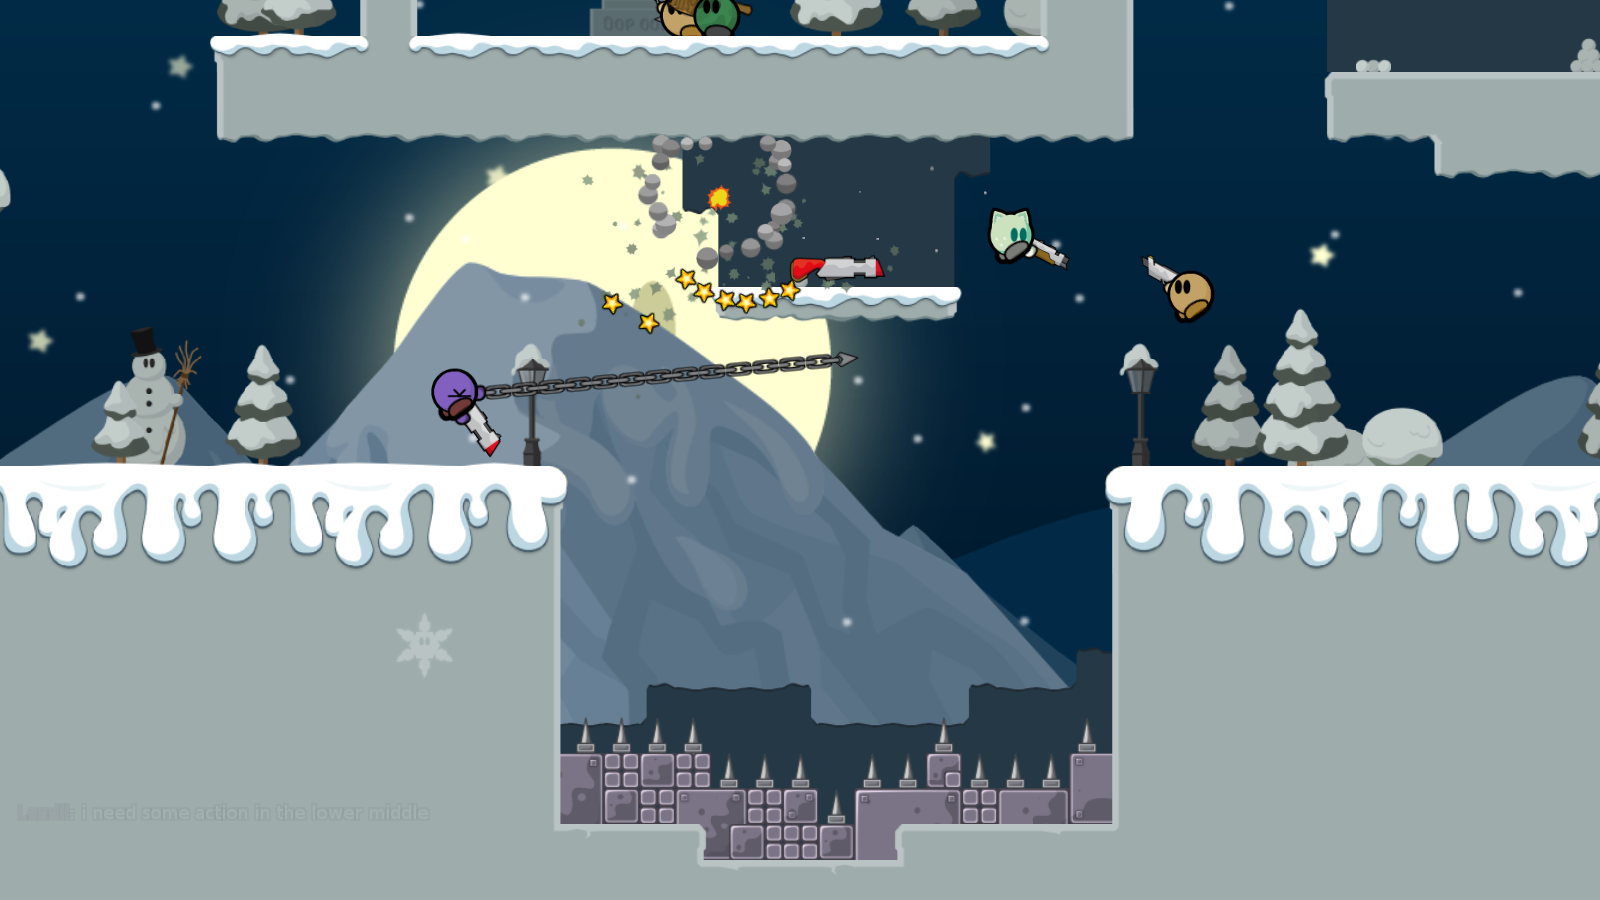
\includegraphics[width=0.7\textwidth]{img/screenshot_winter (1).png}
		      \caption{Entorno gráfico de Teeworlds \cite{teeworlds}}
		      \label{fig:teeworlds}
	      \end{figure}

	      Las características que hemos podido identificar este entorno son las siguientes:
	      \begin{itemize}
		      \item Obliga a la cooperación.
		      \item Obliga a la competición.
		      \item Está limitado a un cierto número de agentes.
	      \end{itemize}

	\item \textbf{Mari0} \cite{mari0} Este juego es una combinación open source entre el mítico Nintendo Super Mario Bros y el Portal de Valve. Esencialmente consiste en las mecánicas del Super Mario, pero este lleva también una pistola de portales. Este juego permite el cooperativo de 4 jugadores y dado el funcionamiento de las pistolas de portales, obliga a la cooperación. El objetivo del entorno es llegar al final de cada mapa. En la figura \ref {fig:mari0} se puede ver la representación gráfica de este entorno.

	      \begin{figure}[ht]
		      \centering
		      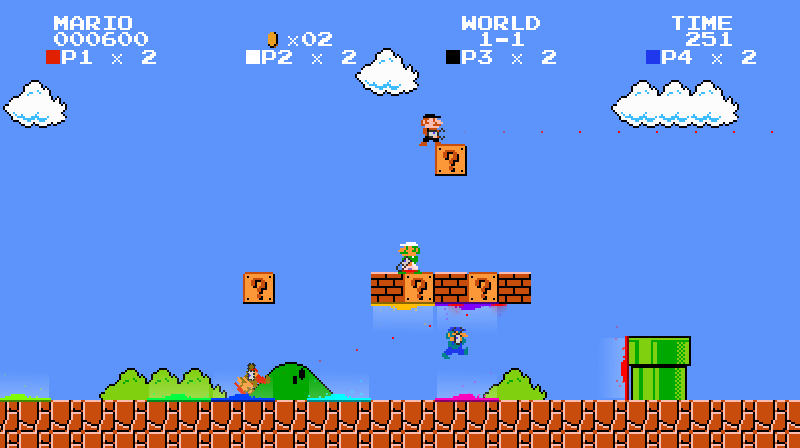
\includegraphics[width=0.7\textwidth]{img/mari0-1.png}
		      \caption{Entorno gráfico de Mari0 \cite{mari0}}
		      \label{fig:mari0}
	      \end{figure}

	      Las características que hemos podido identificar este entorno son las siguientes:
	      \begin{itemize}
		      \item Obliga a la cooperación.
		      \item Está limitado a un cierto número de agentes.
	      \end{itemize}

	\item \textbf{The Battle for Wesnoth} \cite{wesnoth} es un juego open source de estrategia por turnos con temática fantástica. El juego da la posibilidad de jugar en modo multijugador con diferentes misiones con distintos objetivos. El juego tiene implementadas muchas mecánicas típicas de los juegos de estrategia y dentro del juego es posible la cooperación y la competición. En la figura \ref {fig:wesnoth} podemos ver la representación gráfica del entorno.

	      Las características que hemos podido identificar este entorno son las siguientes:
	      \begin{itemize}
		      \item Da posibilidad a la cooperación.
		      \item Da la posibilidad a la competición.
		      \item Está limitado a un cierto número de agentes.
	      \end{itemize}

	      \begin{figure}[ht]
		      \centering
		      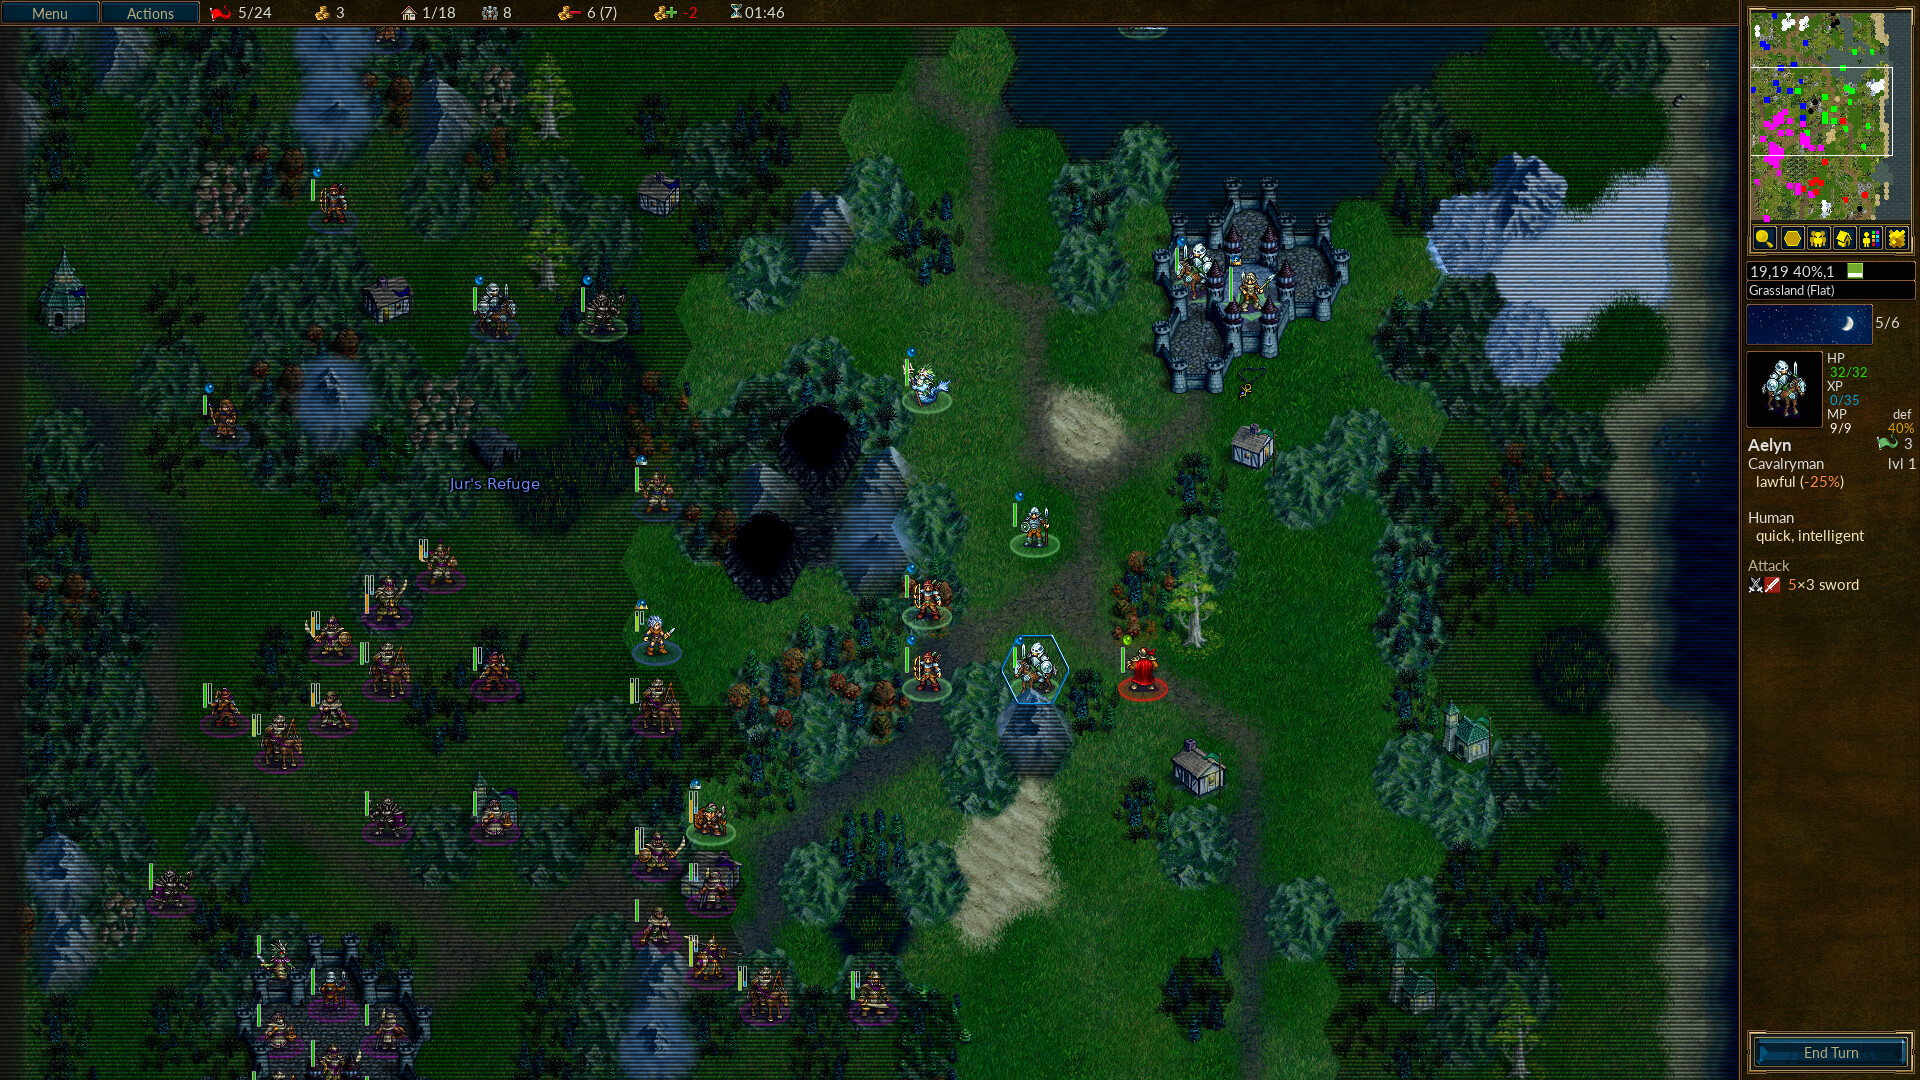
\includegraphics[width=0.7\textwidth]{img/wesnoth-1.16.0-4.jpg}
		      \caption{Entorno gráfico de The Battle for Wesnoth \cite{wesnoth}}
		      \label{fig:wesnoth}
	      \end{figure}

	\item \textbf{Sol Standard} \cite{sol-standard} es un juego open source orientado al jugador vs jugador por turnos que enfrenta a dos jugadores en un combate táctico. Hay 12 clases distintas con diferentes habilidades además de criaturas controladas por IA. Además hay una gran cantidad de ítems y elementos del mapa que permiten estrategias complejas. En la figura \ref {fig:sol-standard} podemos ver la representación gráfica del entorno.

	      Las características que hemos podido identificar este entorno son las siguientes:
	      \begin{itemize}
		      \item Obliga la competición.
		      \item Está limitado a un cierto número de agentes.
	      \end{itemize}

	      \begin{figure}[ht]
		      \centering
		      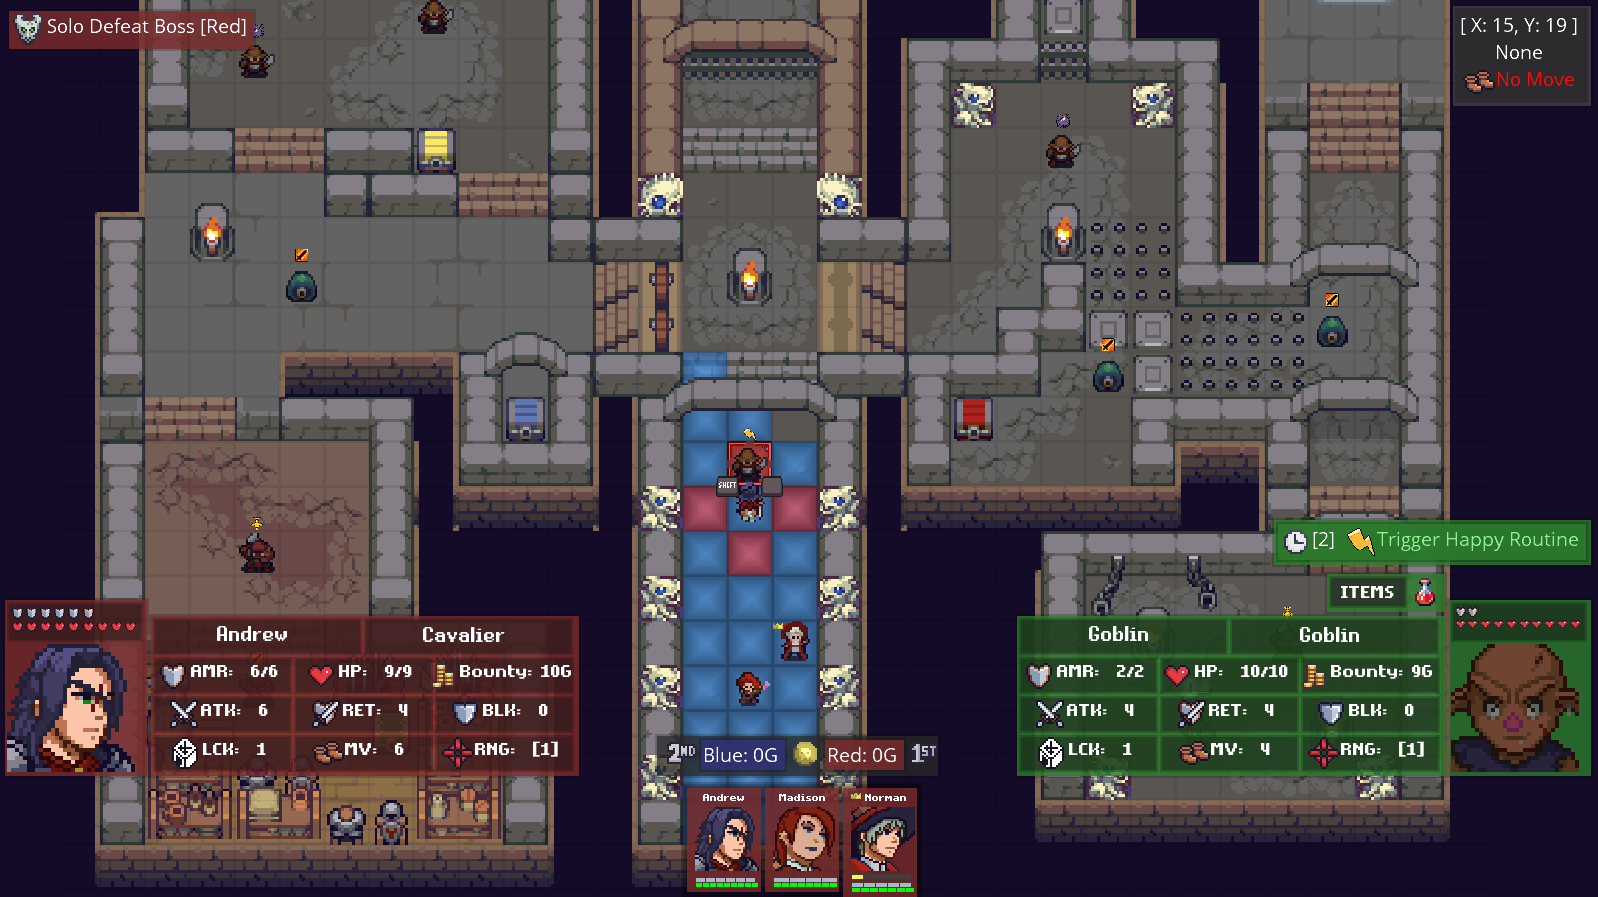
\includegraphics[width=0.7\textwidth]{img/dungeon-map-02.png}
		      \caption{Entorno gráfico de Sol Standard \cite {sol-standard}}
		      \label{fig:sol-standard}
	      \end{figure}

\end{itemize}

\section{Librerías MARL}
Además de los entornos presentados anteriormente, también existen librerías que contienen muchos entornos simples que pueden ser también interesantes. Estas librerías contienen demasiados entornos como para enumerarlos todos, así que los más interesantes los hemos ya descrito en el apartado anterior.

\begin{itemize}
	\item \textbf{Conjunto de entornos por \textit{Jiang, Shuo and Amato, Christopher}} \cite {jiang-repo} Este consiste en un conjunto de entornos que poseen muy buena documentación, pero son muy poco conocidos.

	\item \textbf{Megastep} \cite {megastep-repo} Es un framework que permite crear entornos de FPS (First person shooter) para miles de agentes orientados para usar GPU.

	\item \textbf{OpenSpiel} \cite {openspiel-repo} Es una colección de entornos utiles para RL.

	\item \textbf{PettingZoo} \cite {petting-repo} es una librería de Python para realizar investigaciones en MARL. Contiene múltiples problemas de este ámbito y sigue la interfaz Gym de OpenAI. Los entornos que incluye son juegos multijugador de Atari 2600, juegos desarrollados por ellos mismos y por parte de terceros. Algunos de ellos contienen tareas simples de comunicación entre agentes.\cite {env-list}


\end{itemize}

\section{Entornos descartados}
Estos entornos se han descartado desde el principio antes de realizar su análisis según las métricas que hemos definido por algún problema o impedimento concreto. Aun así los listamos porque también forman parte del estado del arte en entornos MARL. Justificaremos también porque los hemos descartado.

\begin{itemize}
	\item \textbf{StarCraft Multi-Agent Challenge} \cite {starcraft-repo}. Lo descartamos puesto que de este entorno ya se ha investigado tanto que se ha conseguido un agente capaz de ganar a jugadores profesionales de este videojuego. En principio no hay mucho interés en modificar este entorno.

	\item \textbf{Deepmind Lab} \cite{deepmind-repo}. Sus entornos no están adecuados a situaciones multiagente, pero aun así es necesario considerarlo, puesto que con ciertas configuraciones es posible usar alguno de sus entornos de esta manera.

	\item \textbf{Derk's Gym} \cite{derk-repo}. Se trata de un entorno que para obtener acceso a su código es necesario la licencia. Aunque podríamos considerarlo, creemos que hay muchas mejores opciones por coste 0.

\end{itemize}

Finalmente en la tabla \ref{tab:funcionales} podemos observar un resumen de las principales características de los entornos funcionales vistos anteriormente y en la tabla \ref{tab:no-funcionales} de los entornos no funcionales.

\begin{table}[h]
	\begin{center}
		\begin{tabular}{| l | c | c | c | c | c | c | c | c | c |}
			\hline
			\textbf{Nombre}               & \textbf{DOC} & \textbf{NEG} & \textbf{COOP} & \textbf{VS} & \textbf{COM-E} & \textbf{COM-N} & \textbf{GYM} & \textbf{LIM} \\ \hline
			\textbf{Neural MMO}           & X            &              &               & X           &                &                & X            & X            \\
			\textbf{Level-Based Foraging} & X            &              & X             &             &                &                & X            & X            \\
			\textbf{PressurePlate}        & X            &              & X             &             &                &                & X            & X            \\
			\textbf{Robot Warehouse}      & X            &              &               &             &                &                & X            & X            \\
			\textbf{Particle Environment} & X            &              & X             & X           & X              &                & X            & X            \\
			\textbf{MALMO}                & X            & X            & X             & X           &               &  X             &             & X            \\
			\textbf{Pommerman}            & X            &              & X             & X           & X              &                &             &              \\
			\textbf{Flatland}             & X            &              & X             &             &                &                &              &              \\
			\textbf{Hanabi}               & X            &              & X             &             & X              &                & X            &              \\
			\textbf{MultiCarRacing}       & X            &              &               & X           &                &                & X            & X            \\
			\textbf{Overcooked}           & X            &              & X             &             &                &                & X            &              \\ \hline
		\end{tabular}
		\caption{Resumen de los entornos funcionales [Elaboración propia]}
		\label{tab:funcionales}
	\end{center}
\end{table}

\begin{table}[h]
	\begin{center}
		\begin{tabular}{| l | c | c | c | c | c | c |}
			\hline
			\textbf{Nombre}                 & \textbf{DOC} & \textbf{NEG} & \textbf{COOP} & \textbf{VS} & \textbf{COM-E} & \textbf{COM-N} \\ \hline
			\textbf{TrinityCore}            &              & X            & X             & X           &                & X              \\
			\textbf{Teeworlds - DDRace}     & X            &              & X             & X           &                & X              \\
			\textbf{Mari0}                  &              &              & X             &             &                &                \\
			\textbf{The Battle for Wesnoth} &  X            &              & X             & X           &                &                \\
			\textbf{Sol Standard}           &              &              &               & X           &                &                \\
			\hline
		\end{tabular}
		\caption{Resumen de los entornos para adaptación [Elaboración propia]}
		\label{tab:no-funcionales}
	\end{center}
\end{table}